\documentclass{beamer}

\usepackage{multicol}
\usepackage{multimedia}
\usepackage{hyperref}


\usetheme[subsectionpage=progressbar]{metropolis}
\setbeamertemplate{section in toc}[sections numbered]
\setbeamertemplate{subsection in toc}[subsections numbered]

\setbeamertemplate{frame numbering}[fraction]
% \useoutertheme{miniframes}
% \useinnertheme{rounded}
% \usefonttheme{metropolis}
\usecolortheme{spruce}
% \setbeamercolor{background canvas}{bg=white}
% \usecolortheme{wolverine}

\makeatletter
\setbeamertemplate{section page}{
  \centering
  \begin{minipage}{22em}
    \raggedright
    \usebeamercolor[fg]{section title}
    \usebeamerfont{section title}
    \thesection.~\insertsectionhead\\[-1ex]
    \usebeamertemplate*{progress bar in section page}
    \par
    \ifx\insertsubsectionhead\@empty\else%
      \usebeamercolor[fg]{subsection title}%
      \usebeamerfont{subsection title}%
      \thesection.\thesubsection~\insertsubsectionhead
      \fi
  \end{minipage}
  \par
  \vspace{\baselineskip}
}
\makeatother

% \hypersetup{pdfstartview={Fit}} % fits the presentation to the window when first displayed

\titlegraphic{\hfill
\includegraphics[width=.6\textwidth]{img/logo.png}}
\title{Processing Large Datasets with R}
\subtitle{Exam presentation (exam 1)}
\author{\large Joris LIMONIER}
% \institute{University of Luxembourg}
\date{December 7, 2021}



\begin{document}
\metroset{block=fill}

\maketitle

\begin{frame}{Table of Contents}
    \tableofcontents
\end{frame}

\section{Exercise 1 - Shiny\\(Movies dataset)}

\begin{frame}{Import and overview the data}
    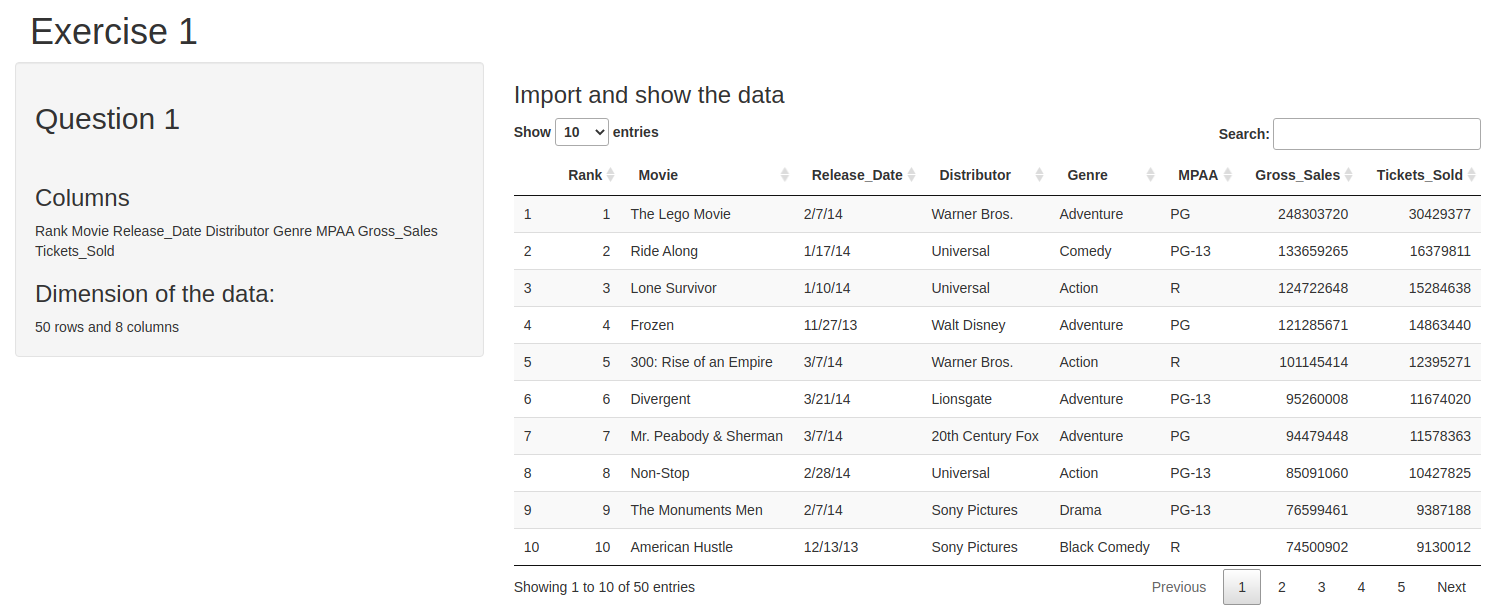
\includegraphics[width=\textwidth]{img/ex1_q1.png}
\end{frame}

\begin{frame}{Plot ticket sales vs gross sales}
    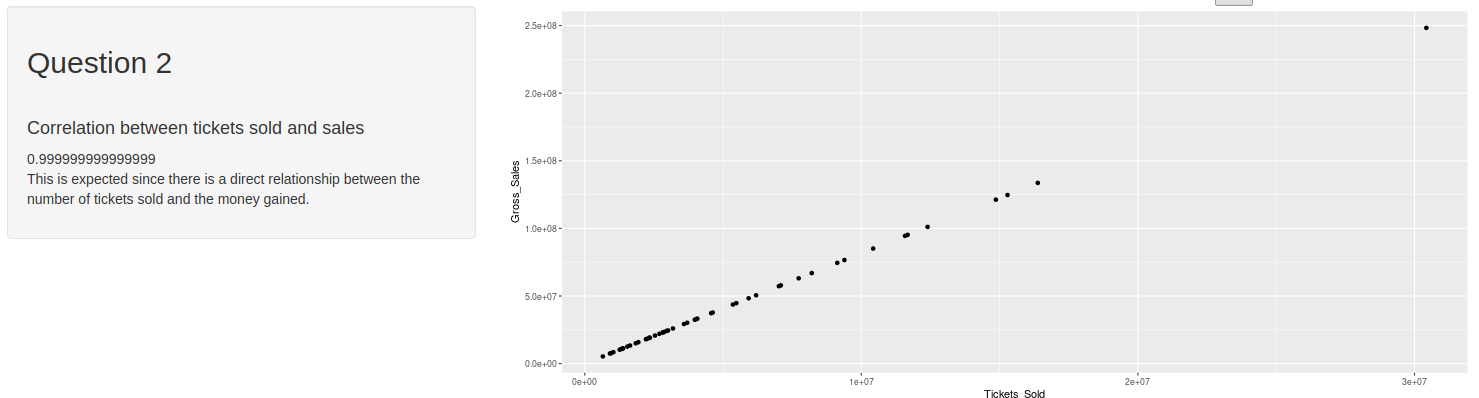
\includegraphics[width=\textwidth]{img/ex1_q2.png}
\end{frame}

\begin{frame}{Box plot and count type of film}
    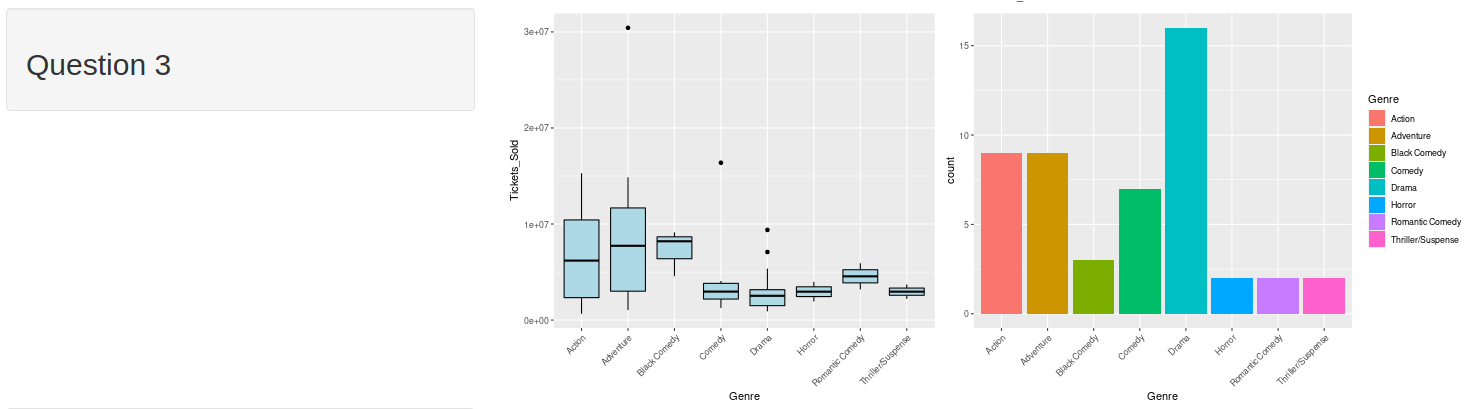
\includegraphics[width=\textwidth]{img/ex1_q3.png}
\end{frame}

\begin{frame}{Tickets sales histogram - play with number of bins}
    \movie[width=\textwidth, height=.8\textheight, loop]{Watch video}{img/R_exam_ex1_q3_animation.mp4}
    \href{https://youtu.be/NTgGG7UvRRU}{Backup link}: \footnotesize https://youtu.be/NTgGG7UvRRU
\end{frame}

\begin{frame}{Tickets and gross sales by genre and distributor}
    \movie[width=\textwidth, height=.8\textheight, loop]{Watch video}{img/R_exam_ex1_q4_animation.mp4}
    \href{https://youtu.be/w\_QQVsRoOpA}{Backup link}: \footnotesize https://youtu.be/w\_QQVsRoOpA
\end{frame}


\section{Exercise 2 - RMarkdown\\(Winter dataset)}
\begin{frame}{Import and overview of the data}
    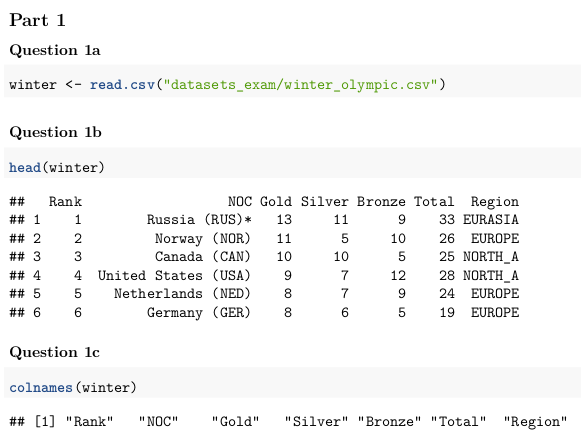
\includegraphics[width=.9\textwidth]{img/ex2_part1_q2.png}
\end{frame}

\begin{frame}{Sort by total medals}
    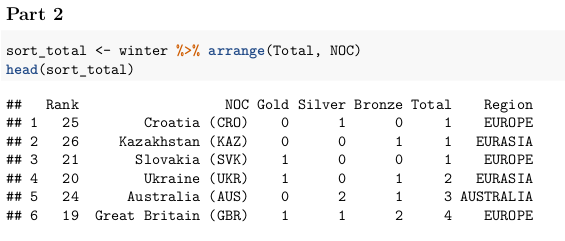
\includegraphics[width=.8\textwidth]{img/ex2_part2.png}
\end{frame}

\begin{frame}{Total and Gold bar plots}
    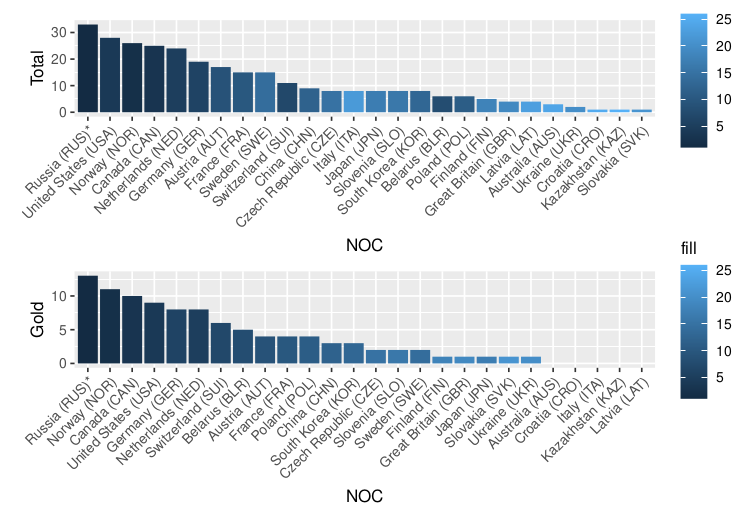
\includegraphics[width=.95\textwidth]{img/ex2_part3_screenshot04.png}
\end{frame}

\begin{frame}{Silver and Bronze bar plots}
    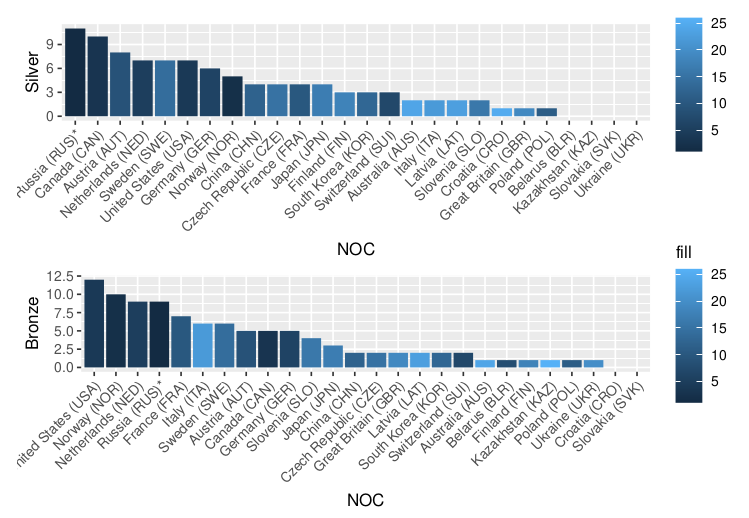
\includegraphics[width=.9\textwidth]{img/ex2_part3_screenshot06.png}
\end{frame}

\begin{frame}{Total of medals}
    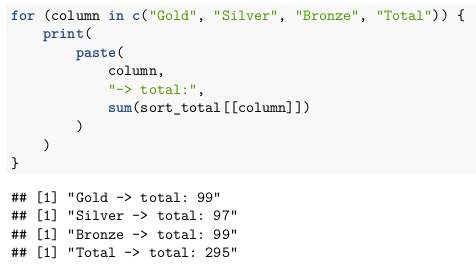
\includegraphics[width=.8\textwidth]{img/ex2_part3_screenshot10.png}
\end{frame}

\begin{frame}{Medians of medals per region}
    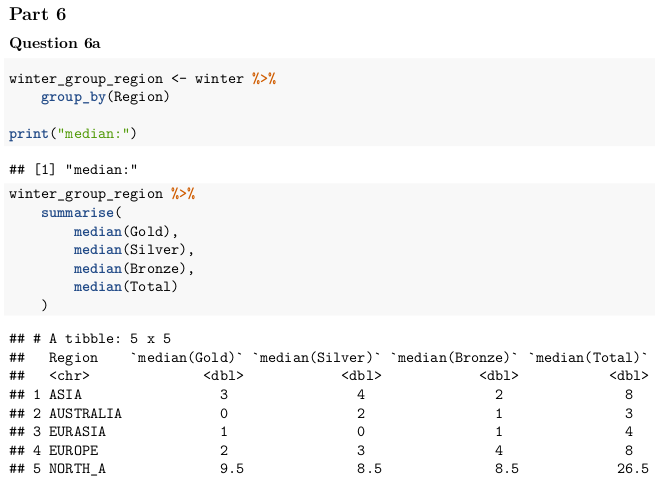
\includegraphics[width=.9\textwidth]{img/ex2_part3_screenshot11.png}
\end{frame}

\begin{frame}{Number of European countries in the dataset}
    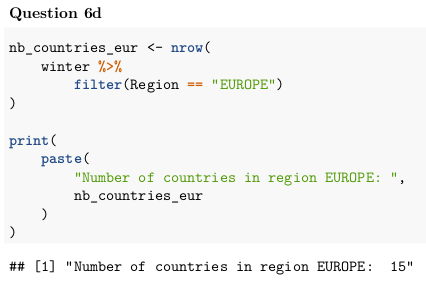
\includegraphics[width=.8\textwidth]{img/ex2_part3_screenshot17.png}
\end{frame}

\begin{frame}{Country with most medals}
    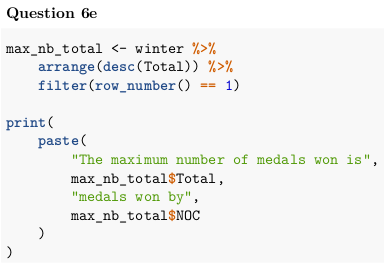
\includegraphics[width=.8\textwidth]{img/ex2_part3_screenshot18.png}
    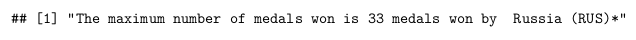
\includegraphics[width=\textwidth]{img/ex2_part3_screenshot19.png}
\end{frame}


\section{Exercise 3 - Data Analysis\\(Summer-Winter dataset)}

\begin{frame}{Import dataset}
    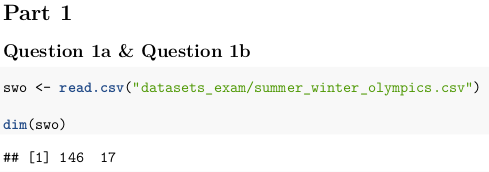
\includegraphics[width=.8\textwidth]{img/ex3_screenshot01.png}
\end{frame}

\begin{frame}{Rename columns}
    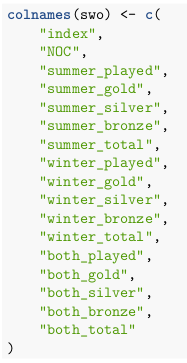
\includegraphics[height=.9\textheight]{img/ex3_screenshot02.png}
\end{frame}

\begin{frame}{Frequency counts}
    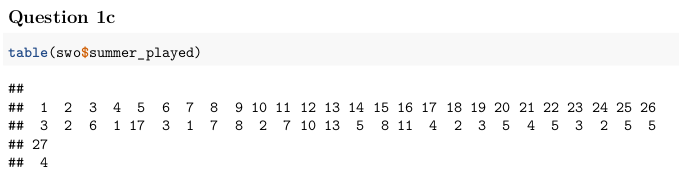
\includegraphics[width=.8\textwidth]{img/ex3_screenshot03.png}
\end{frame}

\begin{frame}{Compare summer vs winter \& played vs total}
    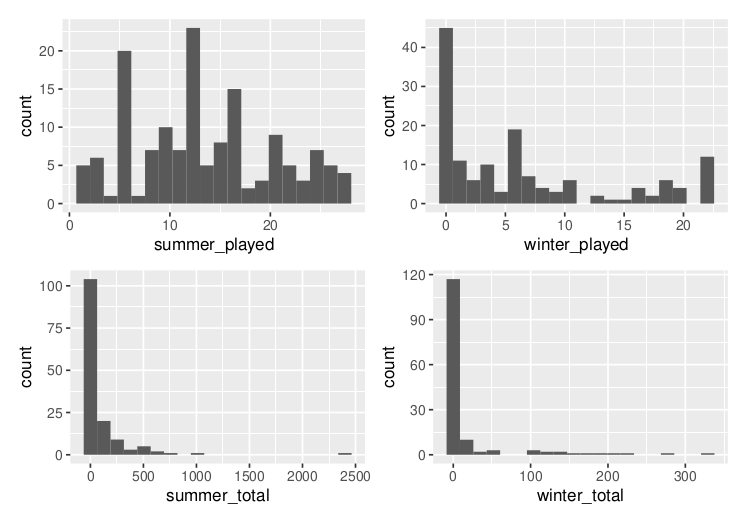
\includegraphics[width=.9\textwidth]{img/ex3_screenshot05.png}
\end{frame}

\begin{frame}{Plot winter vs summer total}
    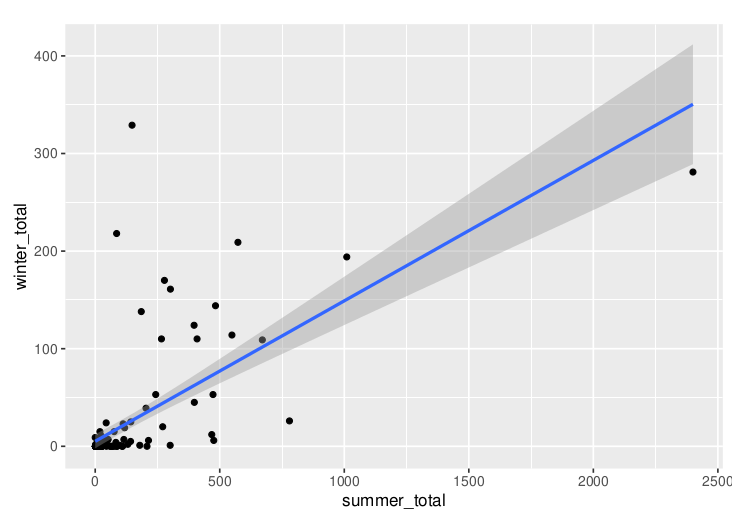
\includegraphics[width=.8\textwidth]{img/ex3_screenshot06.png}
\end{frame}

\begin{frame}{Correlation between winter vs summer total}
    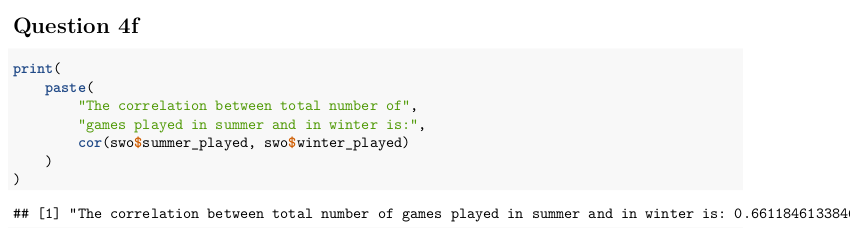
\includegraphics[width=\textwidth]{img/ex3_screenshot07.png}
\end{frame}

\begin{frame}[standout]
    Thank you
    \vfill
    Questions?
\end{frame}

\end{document}